\appendix

\subsection{Model Overview (Continued)}
	\begin{figure}
		\centering
		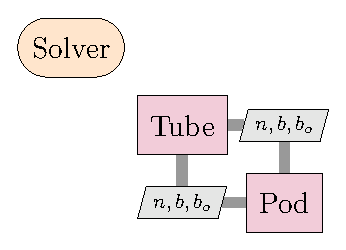
\includegraphics{../images/xdsm/tube_and_pod.pdf}
		\caption{XDSM diagram for entire system model}
		\label{fig:xdsm:toplevel}
	\end{figure}}

\section{TubeGroup}
	\begin{figure}
		\centering
		\includegraphics{../images/tube.png}
		\caption{Hierarchial tree digram showing structure of TubeGroup}
		\label{fig:tree:tube}
	\end{figure}
	\begin{figure}
		\centering
		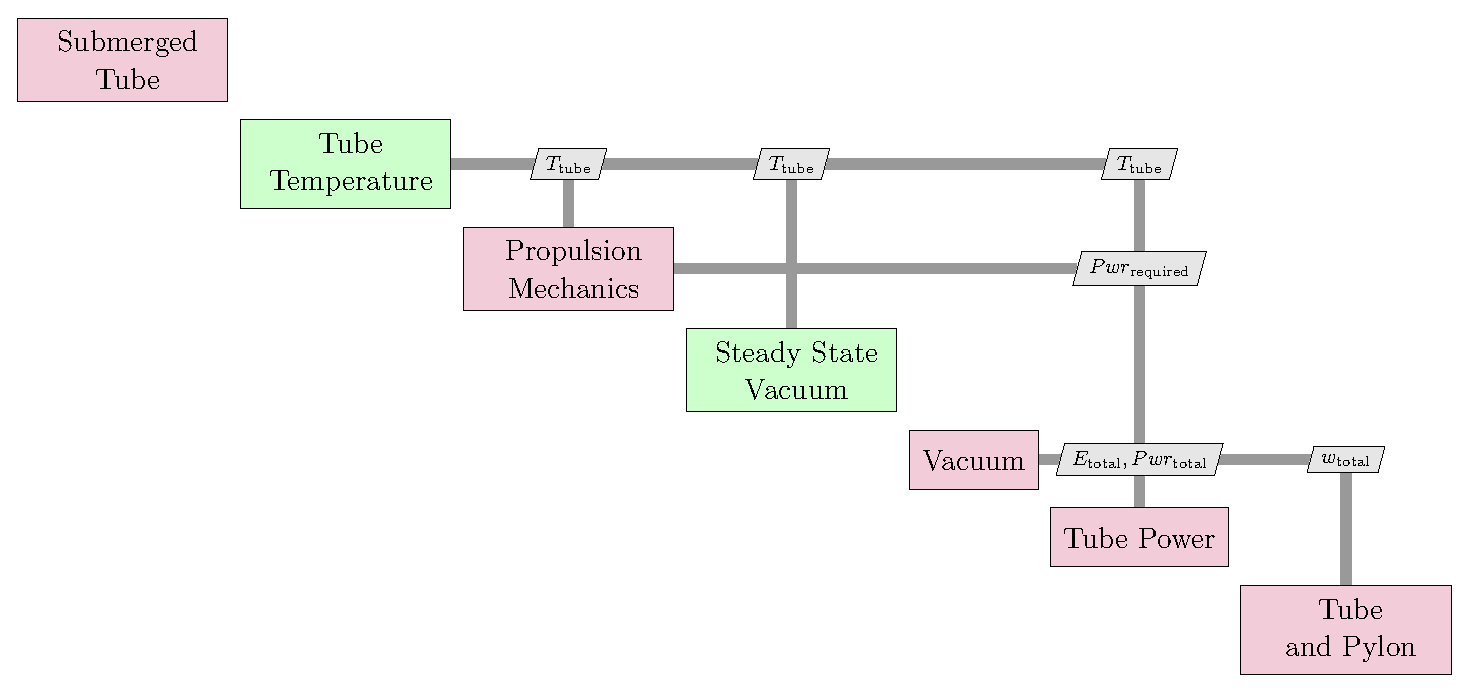
\includegraphics{../images/xdsm/tube.pdf}
		\caption{XDSM diagram for Tube group}
		\label{fig:xdsm:drivetrain}
	\end{figure}}
	\subsection{PropulsionMechanics}
	\subsection{TubeTemp}
		\begin{figure}
			\centering
			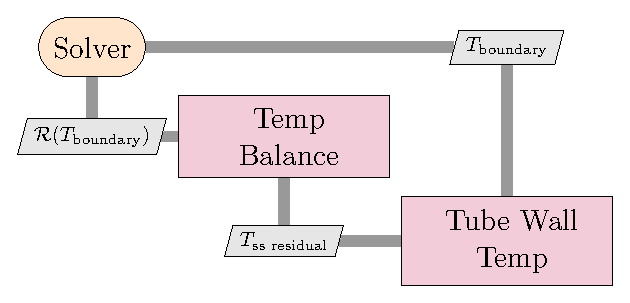
\includegraphics{../images/xdsm/temp.pdf}
			\caption{XDSM diagram for TubeTemp group}
			\label{fig:xdsm:tubetemp}
		\end{figure}}
		\subsubsection{TubeWallTemp}
		\subsubsection{TempBalance}
	\subsection{Vacuum}
		\subsubsection{SteadyStateVacuum}
			\begin{figure}
				\centering
				\includegraphics{../images/xdsm/steady_state_vacuum.pdf}
				\caption{XDSM diagram for SteadyStateVacuum group}
				\label{fig:xdsm:steadystatevacuum}
			\end{figure}}
			\subsubsubsection{FlowStart}
			\subsubsubsection{Compressor}
		\subsubsection{PumpDown}
	\subsection{TubePower}
		\subimport{model_overview/}{tube_power}
	\subsection{Structure}
		\subsubsection{SubmergedTube}
		\subsubsection{TubeAndPylon}
\section{PodGroup}
	\begin{figure}
		\centering
		\includegraphics{../images/pod.png}
		\caption{Hierarchial tree digram showing structure of PodGroup}
		\label{fig:tube}
	\end{figure}
	\begin{figure}
		\centering
		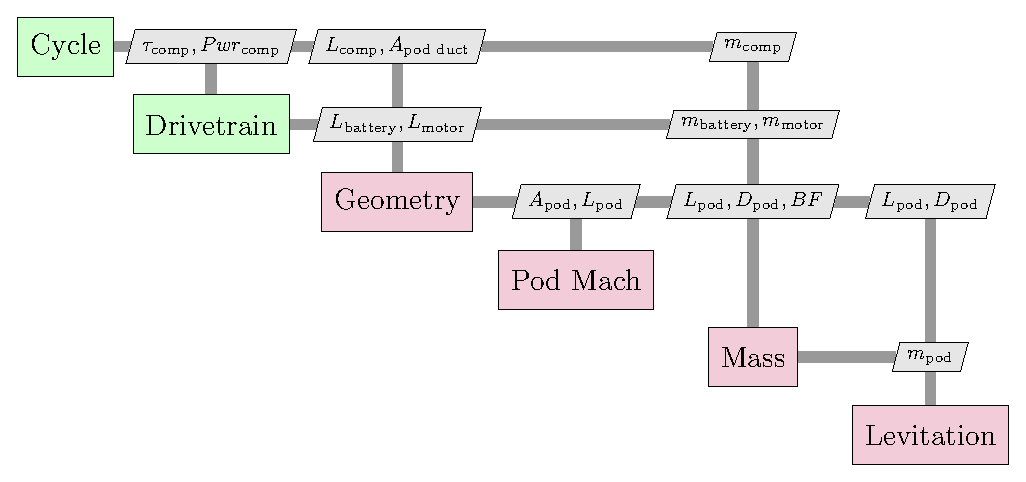
\includegraphics{../images/xdsm/pod.pdf}
		\caption{XDSM diagram for Pod group}
		\label{fig:xdsm:pod}
	\end{figure}}
	\subsection{Drivetrain}
		\begin{figure}
			\centering
			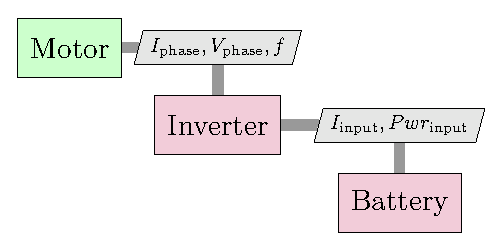
\includegraphics{../images/xdsm/drivetrain.pdf}
			\caption{XDSM diagram for Drivetrain group}
			\label{fig:xdsm:drivetrain}
		\end{figure}
		\subsubsection{Motor}
			\begin{figure}
				\centering
				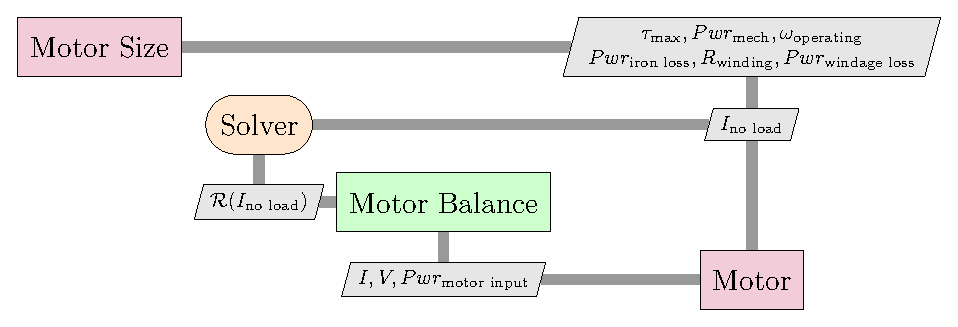
\includegraphics{../images/xdsm/motor.pdf}
				\caption{XDSM diagram for Motor group}
				\label{fig:xdsm:motor}
			\end{figure}}
			\subsubsubsection{MotorSize}
			\subsubsubsection{MotorBalance}
			\subsubsubsection{Motor}
		\subsubsection{Inverter}
		\subsubsection{Battery}
	\subsection{PodGeometry}
	\subsection{Cycle}
		\begin{figure}
			\centering
			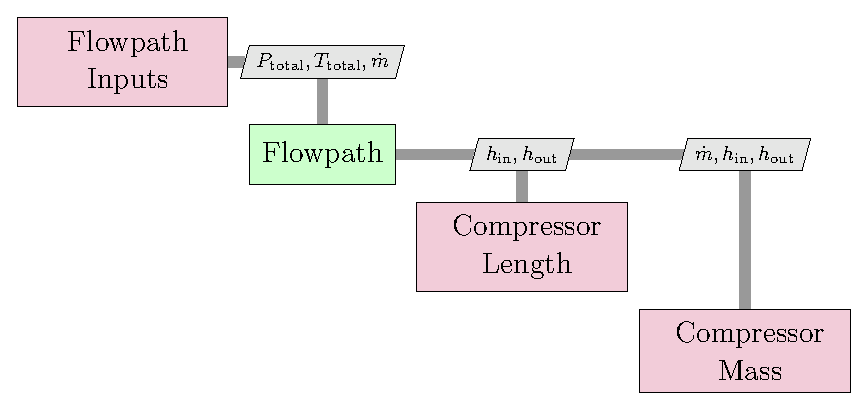
\includegraphics{../images/xdsm/cycle.pdf}
			\caption{XDSM diagram for Cycle group}
			\label{fig:xdsm:cycle}
		\end{figure}
		\subsubsection{Flowpath}
			\begin{figure}
				\centering
				\includegraphics{../images/xdsm/flowpath.pdf}
				\caption{XDSM diagram for Flowpath group}
				\label{fig:xdsm:flowpath}
			\end{figure}}
			\subsubsubsection{CompressorLength}
			\subsubsubsection{CompressorMass}
			\subsubsubsection{FlowpathInputs}
			\ssubsection{LevGroup}
			\begin{figure}
				\centering
				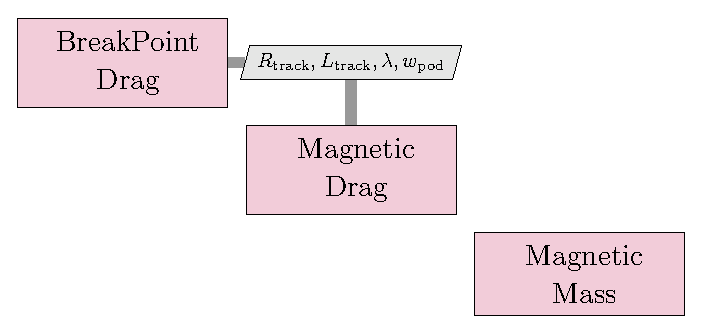
\includegraphics{../images/xdsm/levitation.pdf}
				\caption{XDSM diagram for the LevGroup group}
				\label{fig:xdsm:levitation}
			\end{figure}}
		\subsubsection{BreakpointDrag}
		\subsubsection{MagneticDrag}
		\subsubsection{MagneticMass}
	\subsection{Drag}
	\subsection{PodMach}
	\subsection{PodMass}
\section{TicketCost}
\section{SampleMission}

% from flight_frequency.tex
\begin{equation}
	\label{eq:linear_acceleration}
	Insert Linear Acceleration Equations
\end{equation}
\end{equation}
Assuming a braking deceleration of 1g, a Mach number of .8, and a tunnel
temperature of 320 K \cite{Chin}, the minimum distance between pods is
calculated to be 4.2 km with no safety margin. At top speed, the deceleration
time is calculated to be 29.2 s.


